\section{Metodologia}

%------------------------------------------------

\begin{frame}{Comprimento de onda de de Broglie}

    de Broglie relaciona o momento de uma partícula $p$, a constante de Planck $h$ e seu comprimento de onda $\lambda$.        
    \begin{equation}
        \lambda = \frac{h}{p}
    \end{equation}

\end{frame}

%------------------------------------------------
\begin{frame}{Metodologia}
    \Huge{\centerline{\textbf{Metodologia}}}
\end{frame}

\begin{frame}{Comparação do comprimento de onda de Bragg e de Broglie}

Queremos comparar o comprimento de onda dos raios X utilizados por Bragg em seus experimentos de difração de cristais com o comprimento de onda de elétrons acelerados a alguns quilovolts, segundo a hipótese de de Broglie, para verificar se a teoria desenvolvida por Bragg é aplicável a esse problema.

\begin{equation}
\begin{aligned}
\lambda &= \frac{h}{p} = \frac{h}{\sqrt{2 m_e e V}} \\[6pt]
        &= \frac{6.63 \times 10^{-34}}
        {\sqrt{2 (9.11 \times 10^{-31})(1.6 \times 10^{-19})(5 \times 10^3)}} \\[6pt]
        &\approx 1.74 \times 10^{-11} \ \text{m}
\end{aligned}
\end{equation}
\end{frame}

\begin{frame}{Difração de DEBYE-SCHERRER}

        \begin{center}
        \begin{figure}
        \caption{Representação do método de difração Debye-Scherrer.}
        \vspace*{-0.25cm}
        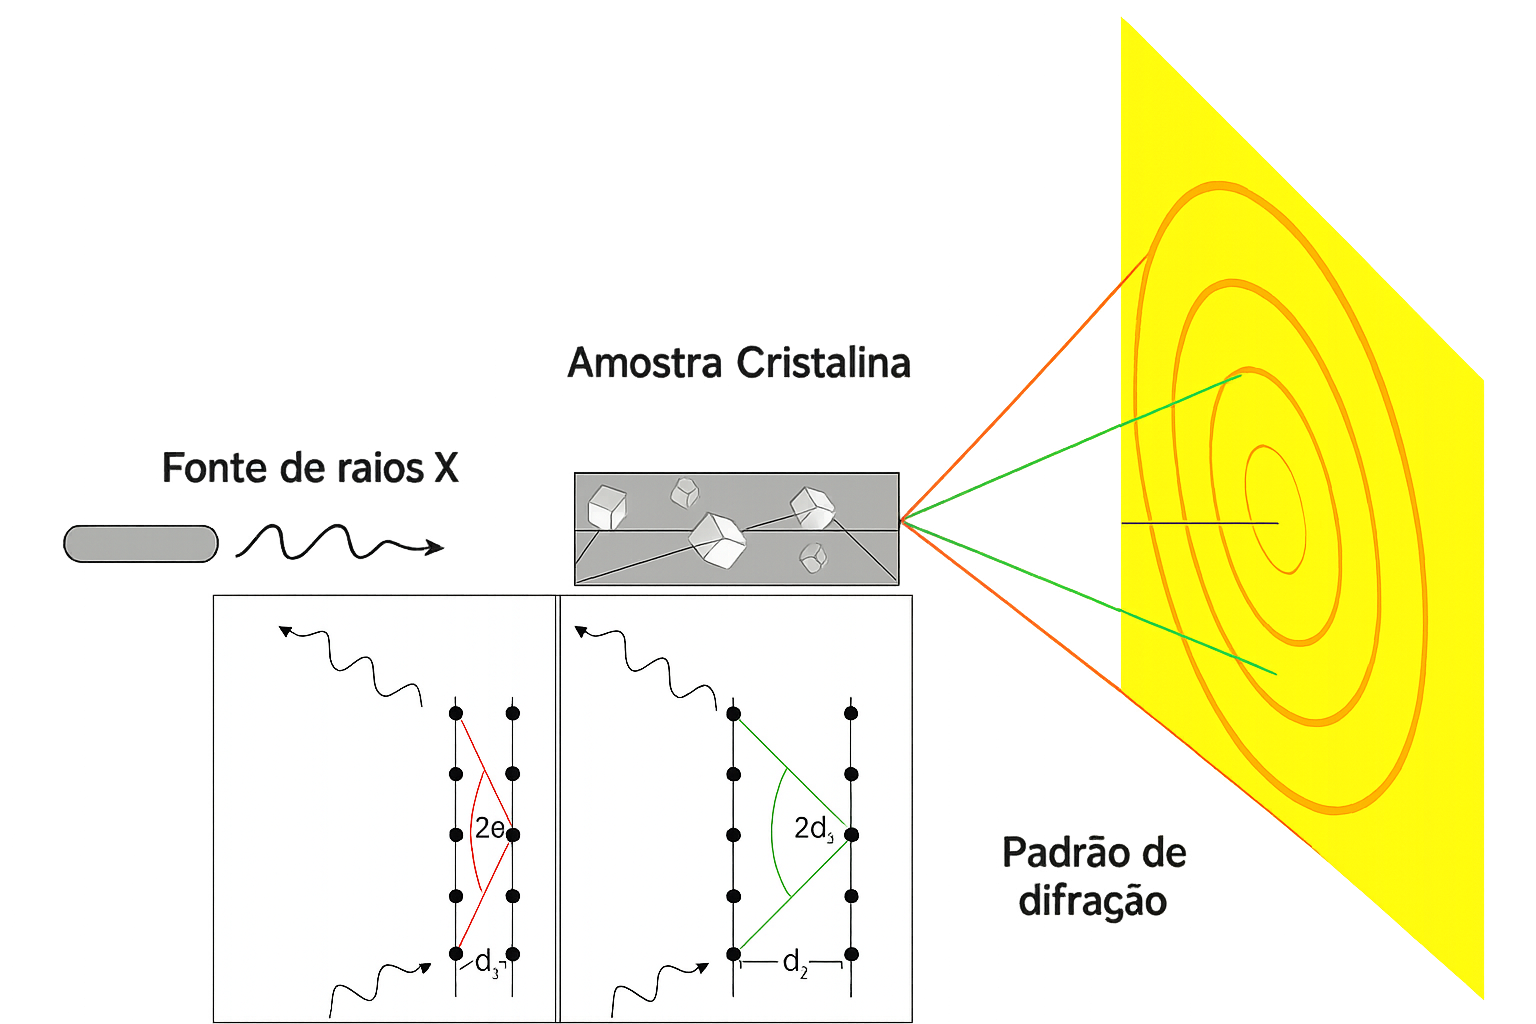
\includegraphics[width=0.75\textwidth,height=0.75\textheight,keepaspectratio]{figuras/debye.png}\par
        {\scriptsize Fonte: Adaptado da Wikipedia.}
        \end{figure}
        \end{center}
    
\end{frame}



\begin{frame}{Diferença entre um policristal e um mono cristal.}

    \begin{columns}[c]
      

        \column{.45\textwidth}
        \begin{figure}
          \centering
          \caption{Representação da estrutura de mono cristais e policristais.}
          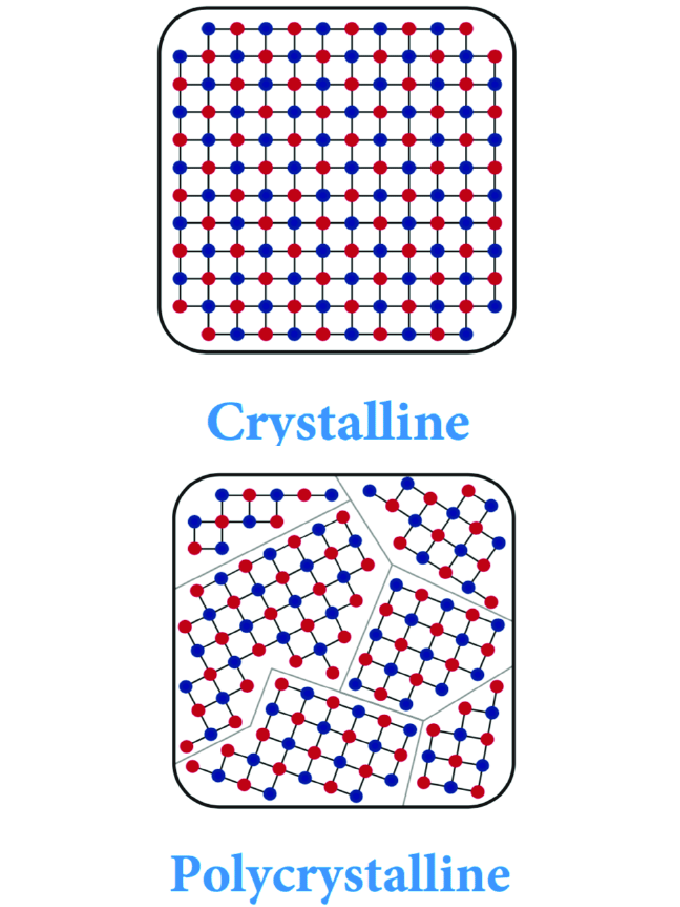
\includegraphics[width=4.10cm]{figuras/poli_mono2.png}\par
          {\scriptsize Fonte: Retirado da internet.}
        \end{figure}

  \column{.45\textwidth}
        Os policristais são sólidos formados por muitos pequenos monocristais com diferentes
orientações.

    \end{columns}

    
\end{frame}

\begin{frame}

        \begin{center}
        \begin{figure}
          \caption{Representação da estrutura de diferentes tipos de cristais.}
        % \vspace*{-0.45cm}
        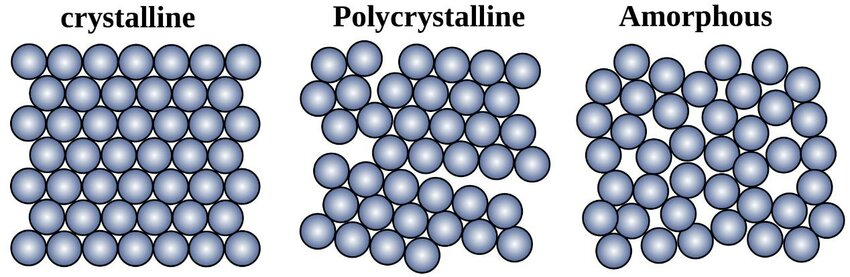
\includegraphics[width=0.75\textwidth,height=0.75\textheight,keepaspectratio]{figuras/poli_mono.jpg}\par
          {\scriptsize Fonte: Retirado da internet.}
        \end{figure}
        \end{center}



    
\end{frame}

\begin{frame}{Policristal de grafite.}

        \begin{center}
        \begin{figure}
        \caption{Exemplo de estrutura de um policristal de grafite.}
        \vspace*{-0.25cm}
        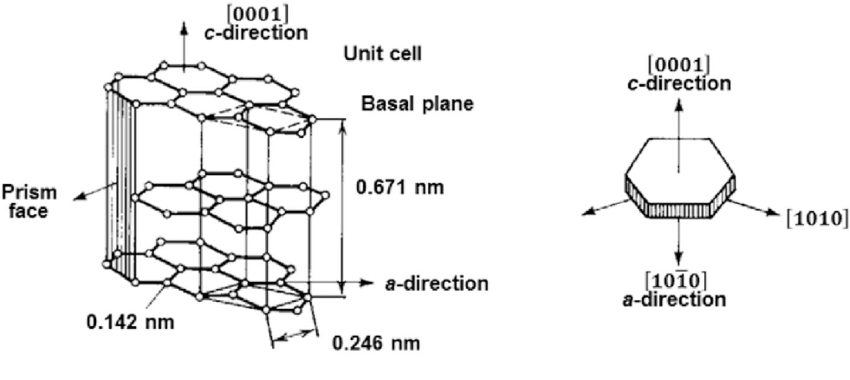
\includegraphics[width=0.75\textwidth,height=0.75\textheight,keepaspectratio]{figuras/Crystallographic-structure-of-graphite.png}\par
        {\scriptsize Fonte: Retirado de \cite{STEFANESCU2016102}.}
        \end{figure}
        \end{center}
    
\end{frame}


\begin{frame}{Equipamento utilizado}

    \begin{columns}[c]
        \column{.45\textwidth}
        \begin{figure}
          \centering
          \caption{Equipamento utilizado (visão frontal).}
          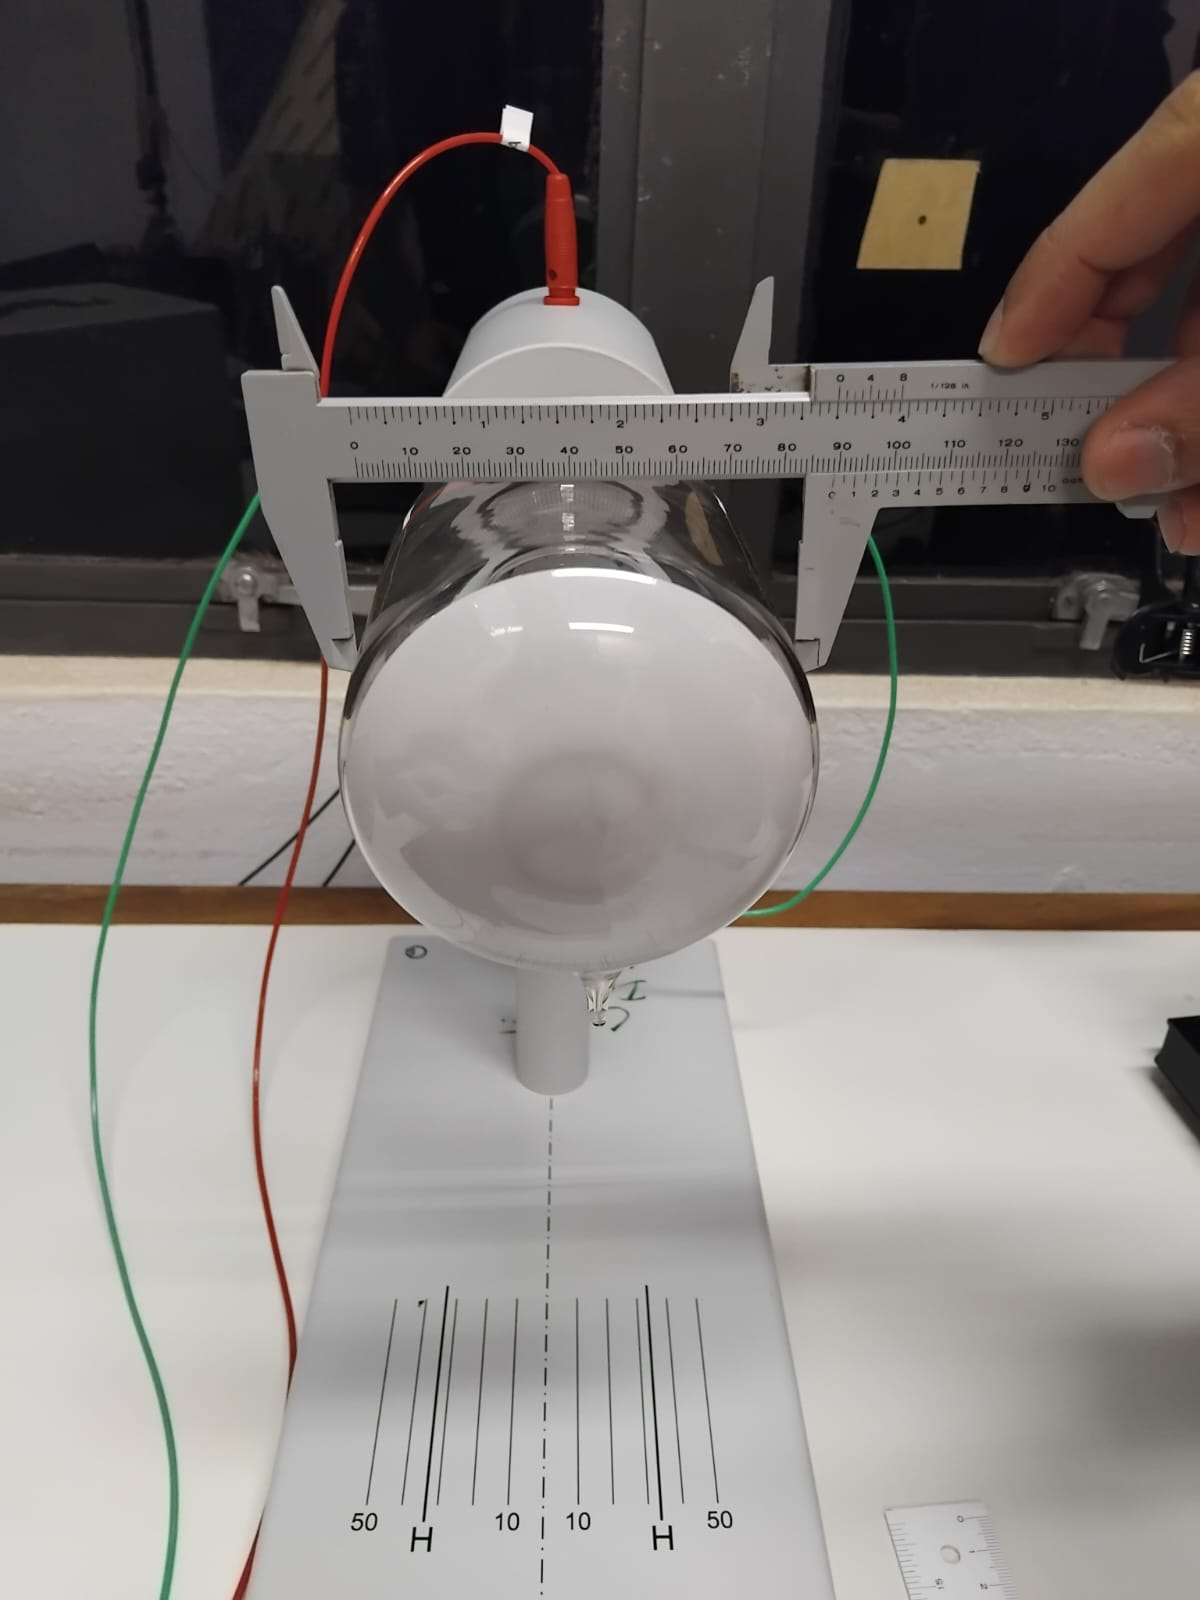
\includegraphics[width=4.25cm]{figuras/metodologia_3.jpeg}\par
          {\scriptsize Fonte: Elaborado pelo autor.}
        \end{figure}

        \column{.45\textwidth}
        \begin{figure}
          \centering
          \caption{Equipamento utilizado (visão lateral).}
          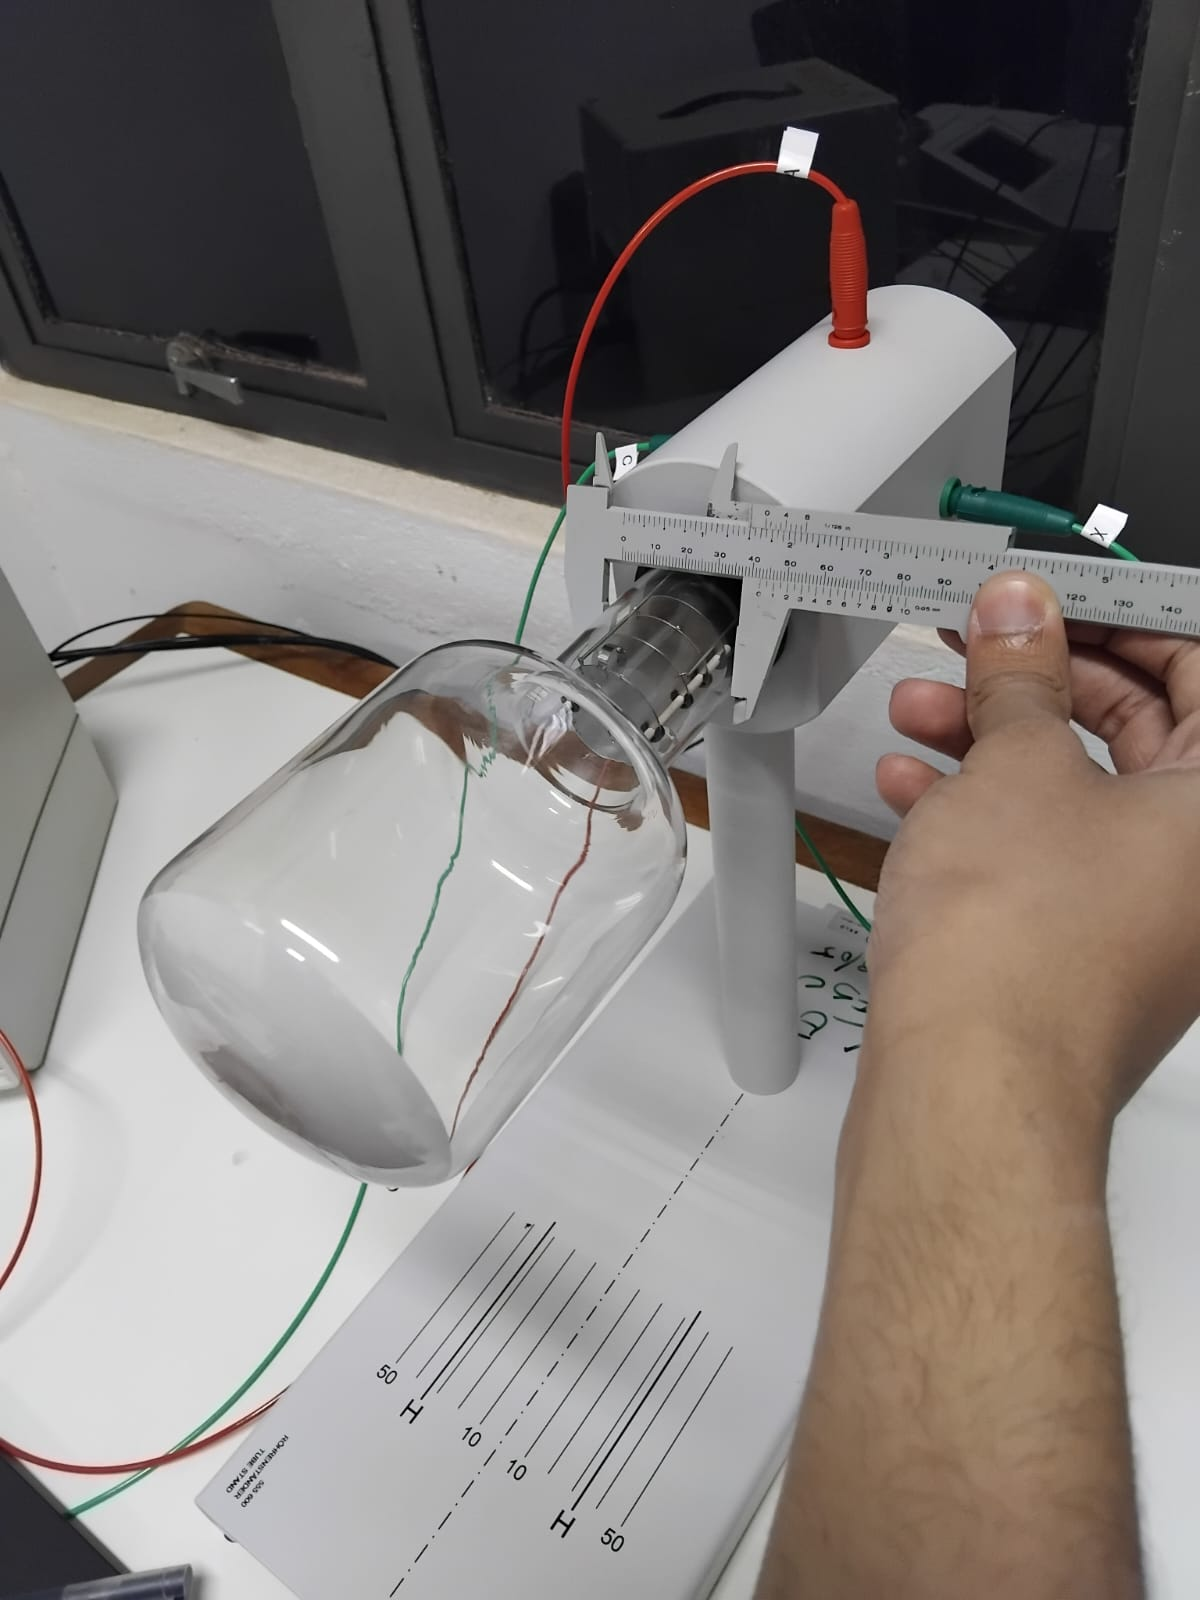
\includegraphics[width=4.25cm]{figuras/metodologia_2.jpeg}\par
          {\scriptsize Fonte: Elaborado pelo autor.}
        \end{figure}

    \end{columns}

    
\end{frame}


\begin{frame}{Difração}

    \begin{columns}[c]
        \column{.45\textwidth}
        \begin{figure}
          \centering
          \caption{Padão de difração observado.}
          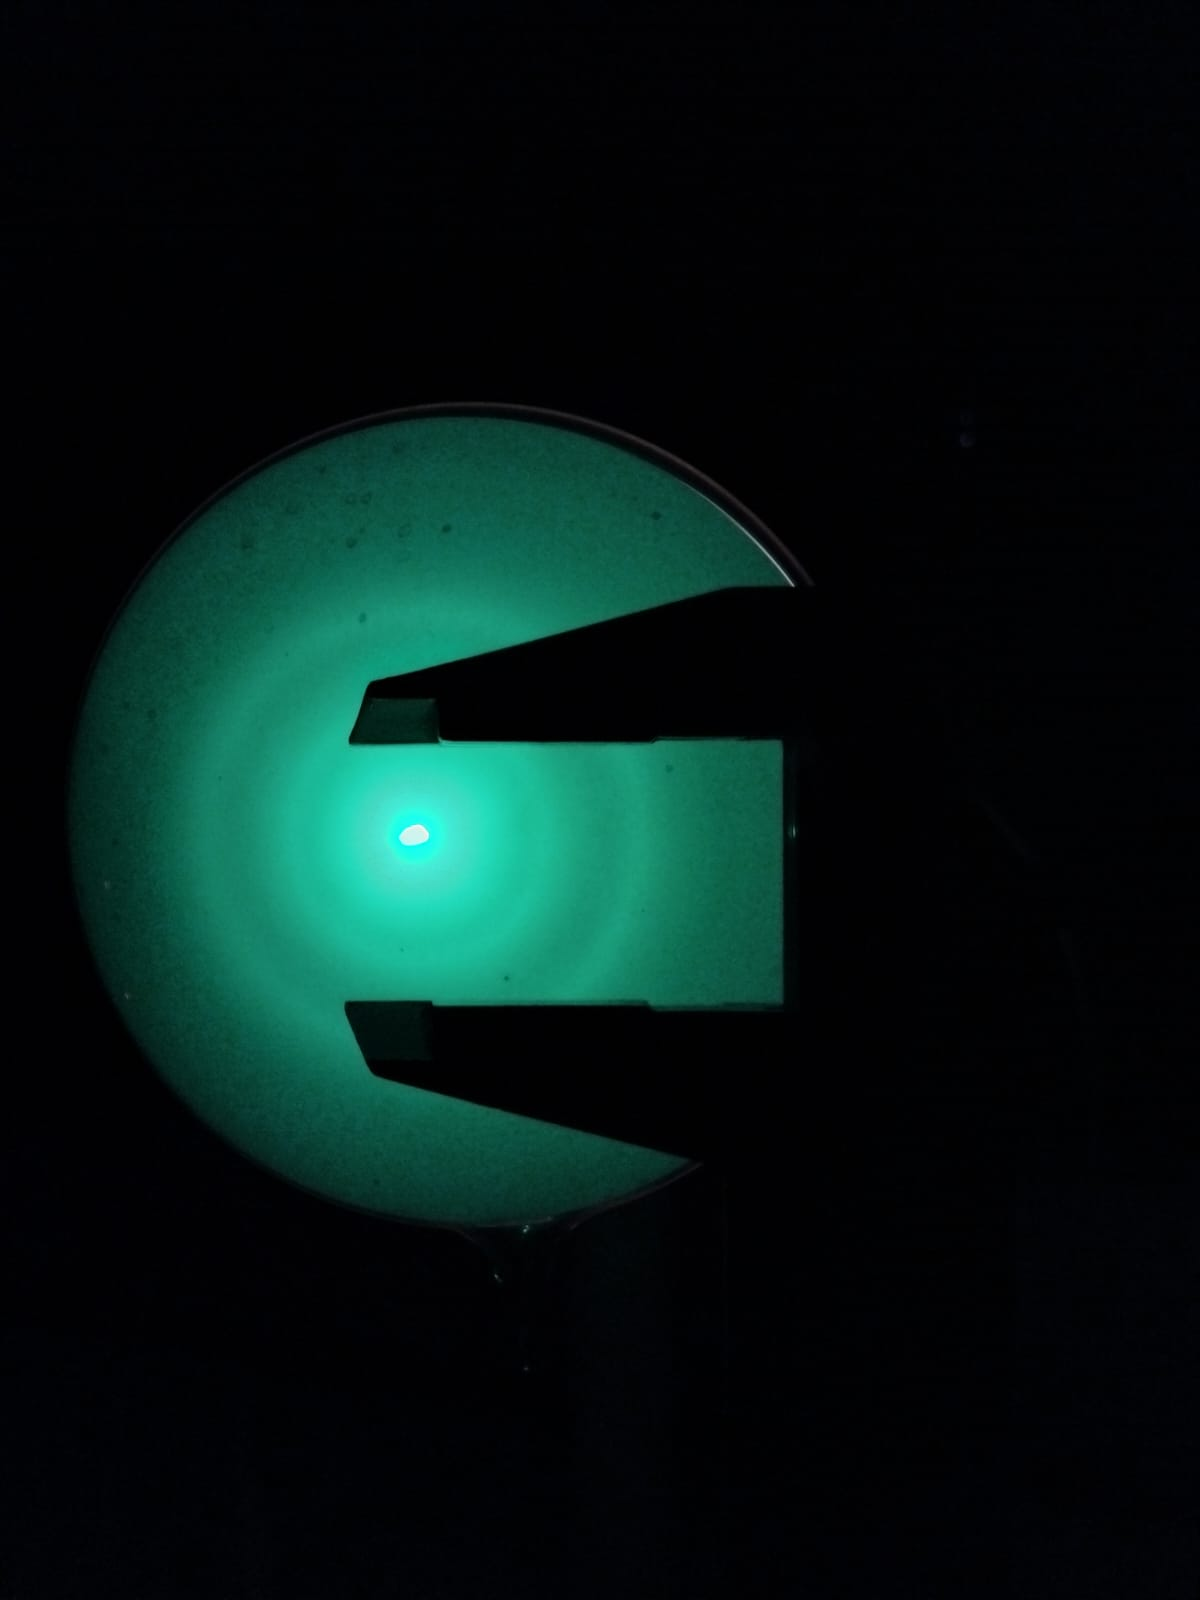
\includegraphics[width=4.25cm]{figuras/metodologia_1.jpeg}\par
        {\scriptsize Fonte: Elabora pelo autor.}
        \end{figure}

        \column{.45\textwidth}
        Padrão de difração observado.
    \end{columns}

    
\end{frame}
